% \newpage
\begin{figure}[!ht]
\begin{minipage}{\textwidth}
\fontsize{8}{8}\fontfamily{pcr}\selectfont
\begin{tabular}{l l}
\textbf{An example from tasks 1}: & \textbf{(requiring one supportive fact to solve)}\\
\\
\textbf{Story}: & \\
& John travelled to the hallway. \\
& Mary journeyed to the bathroom. \\
& Daniel went back to the bathroom. \\
& John moved to the bedroom \\
\\
\textbf{Question}: & \\
& Where is Mary? \\
\textbf{Model's output}: & \\
& bathroom
\end{tabular}
\end{minipage}
\\ \vfill
\vspace{20pt} % maximize space between the minipages
\begin{minipage}{\textwidth}
    \centering
    \begin{subfigure}[t]{\textwidth}
        \centering
        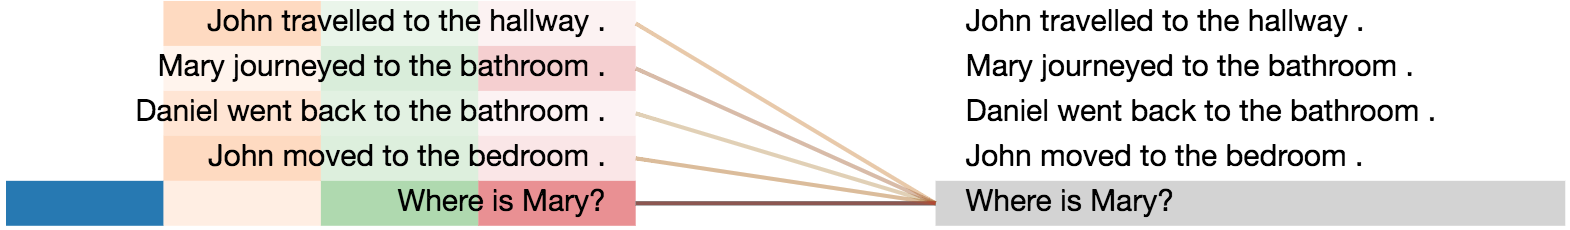
\includegraphics[height=0.8in]{04-part-03/chapter-06/figs_and_tables/figs_attention_babi/e1-step1.png}
        \caption{Step 1}
    \end{subfigure}%
    \hfill \hfill
    \begin{subfigure}[t]{\textwidth}
        \centering
        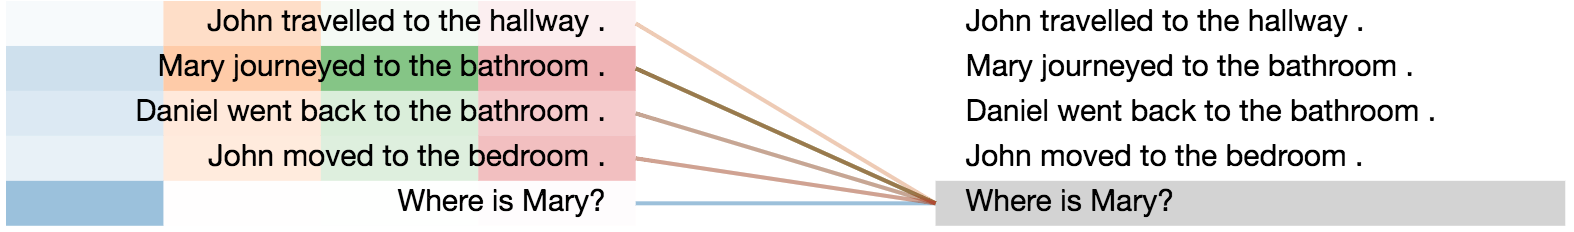
\includegraphics[height=0.8in]{04-part-03/chapter-06/figs_and_tables/figs_attention_babi/e1-step2}
        \caption{Step 2}
    \end{subfigure}
    \hfill \hfill
    \begin{subfigure}[t]{\textwidth}
        \centering
        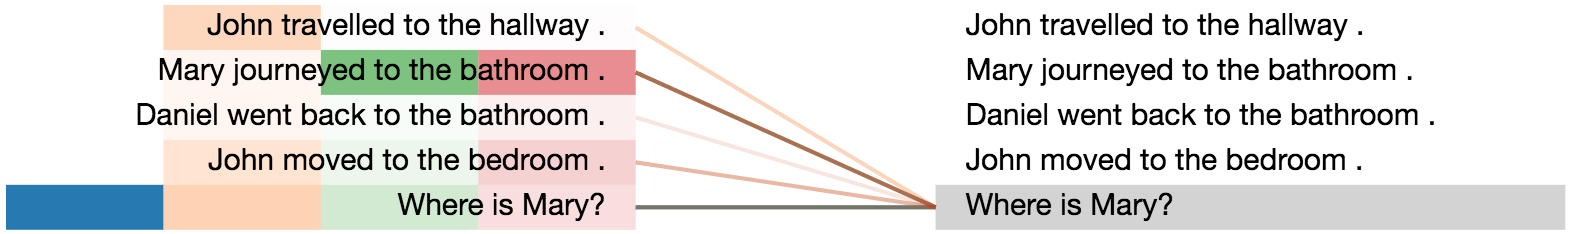
\includegraphics[height=0.8in]{04-part-03/chapter-06/figs_and_tables/figs_attention_babi/e1-step3}
        \caption{Step 3}
    \end{subfigure}
    \hfill \hfill 
    \begin{subfigure}[t]{\textwidth}
        \centering
        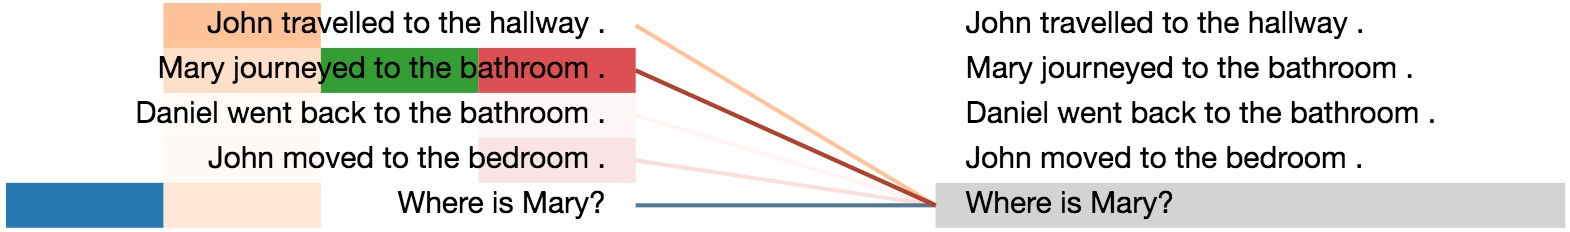
\includegraphics[height=0.8in]{04-part-03/chapter-06/figs_and_tables/figs_attention_babi/e1-step4}
        \caption{Step 4}
    \end{subfigure}
\end{minipage}
    \caption{\label{fig:ex1}Visualization of the attention distributions, when encoding the question: \emph{``Where is Mary?''}.}
\end{figure}
\afterpage{\clearpage}




\begin{figure}[!h]
\begin{minipage}{\textwidth}
\fontsize{8}{8}\fontfamily{pcr}\selectfont
\begin{tabular}{l l}
\textbf{An example from tasks 2}: & \textbf{(requiring two supportive facts to solve)}\\
\\
\textbf{Story}: & \\
& Sandra journeyed to the hallway. \\
& Mary went to the bathroom. \\
& Mary took the apple there. \\
& Mary dropped the apple. \\
\\
\textbf{Question}: & \\
& Where is the apple? \\
\textbf{Model's output}: & \\
& bathroom
\end{tabular}
\end{minipage}
\\  \vfill
\vspace{20pt} % maximize space between the minipages
\begin{minipage}{\textwidth}
    \centering
    \begin{subfigure}[t]{\textwidth}
        \centering
        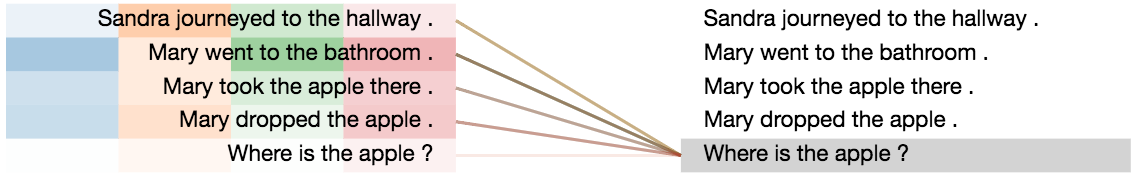
\includegraphics[height=0.8in]{04-part-03/chapter-06/figs_and_tables/figs_attention_babi/e2-step1}
        \caption{Step 1}
    \end{subfigure}%
    \hfill \hfill
    \begin{subfigure}[t]{\textwidth}
        \centering
        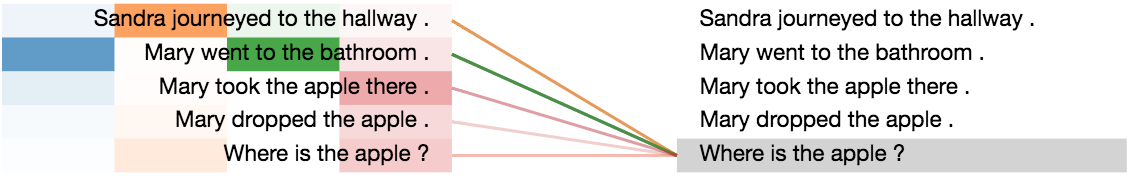
\includegraphics[height=0.8in]{04-part-03/chapter-06/figs_and_tables/figs_attention_babi/e2-step2}
        \caption{Step 2}
    \end{subfigure}
    \hfill \hfill
    \begin{subfigure}[t]{\textwidth}
        \centering
        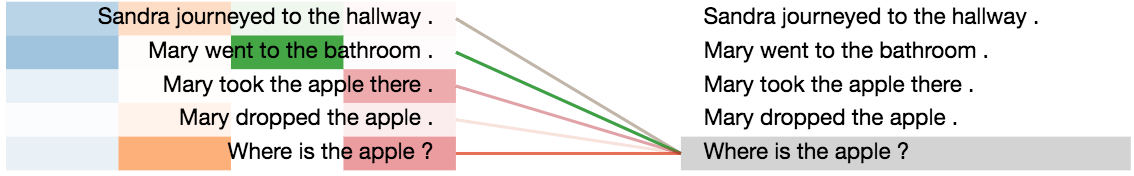
\includegraphics[height=0.8in]{04-part-03/chapter-06/figs_and_tables/figs_attention_babi/e2-step3}
        \caption{Step 3}
    \end{subfigure}
    \hfill \hfill 
    \begin{subfigure}[t]{\textwidth}
        \centering
        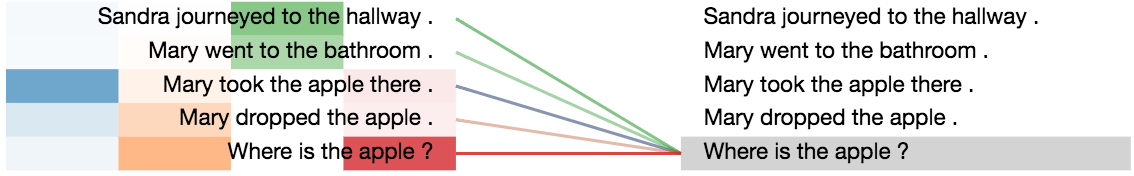
\includegraphics[height=0.8in]{04-part-03/chapter-06/figs_and_tables/figs_attention_babi/e2-step4}
        \caption{Step 4}
    \end{subfigure}
    \end{minipage}
    \caption{\label{fig:ex2}Visualization of the attention distributions, when encoding the question: \emph{``Where is the apple?''}.}
\end{figure}

\afterpage{\clearpage}

\begin{figure}[!h]
\begin{minipage}{\textwidth}
\fontsize{8}{8}\fontfamily{pcr}\selectfont
\begin{tabular}{l l}
\textbf{An example from tasks 2}: & \textbf{(requiring two supportive facts to solve)}\\
\\
\textbf{Story}: & \\
& John went to the hallway. \\
& John went back to the bathroom. \\
& John grabbed the milk there. \\
& Sandra went back to the office. \\
& Sandra journeyed to the kitchen. \\
& Sandra got the apple there. \\
& Sandra dropped the apple there. \\
& John dropped the milk. \\
\\
\textbf{Question}: & \\
& Where is the milk? \\
\textbf{Model's output}: & \\
& bathroom
\end{tabular}
\end{minipage}
\\ \vfill
\vspace{20pt} % maximize space between the minipages
\begin{minipage}{\textwidth}
    \centering
    \begin{subfigure}[t]{\textwidth}
        \centering
        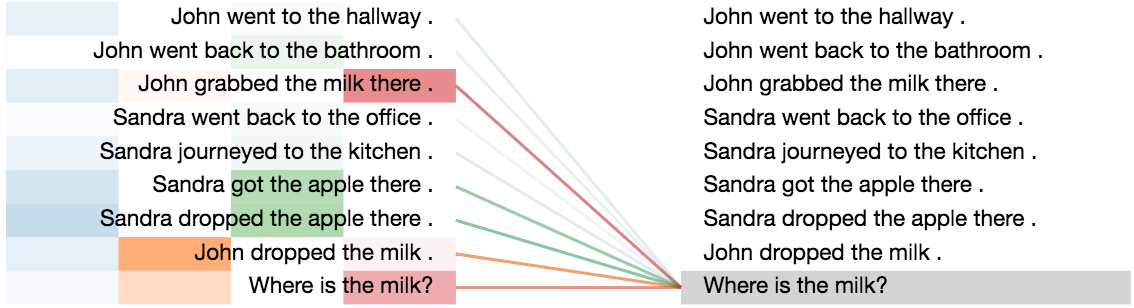
\includegraphics[height=1.3in]{04-part-03/chapter-06/figs_and_tables/figs_attention_babi/e3-step1}
        \caption{Step 1}
    \end{subfigure}%
    \hfill \hfill
    \begin{subfigure}[t]{\textwidth}
        \centering
        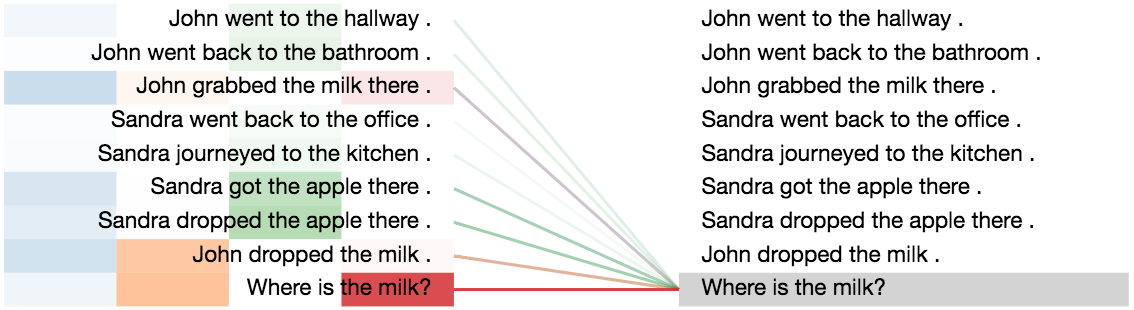
\includegraphics[height=1.3in]{04-part-03/chapter-06/figs_and_tables/figs_attention_babi/e3-step2}
        \caption{Step 2}
    \end{subfigure}
    \hfill \hfill
    \begin{subfigure}[t]{\textwidth}
        \centering
        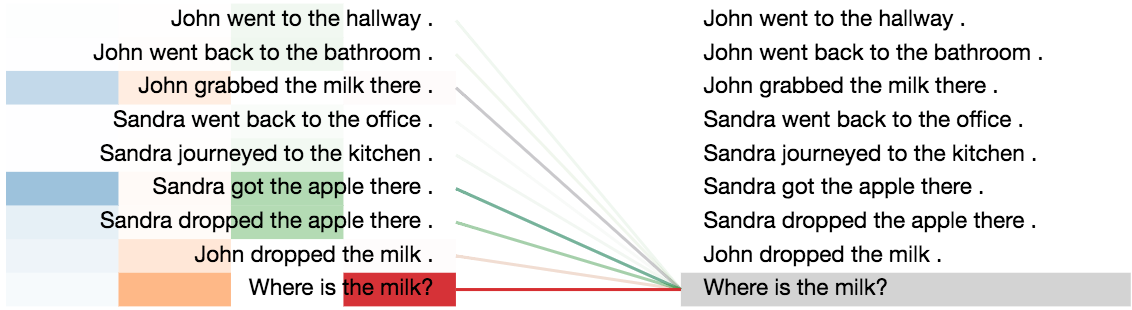
\includegraphics[height=1.3in]{04-part-03/chapter-06/figs_and_tables/figs_attention_babi/e3-step3}
        \caption{Step 3}
    \end{subfigure}
    \hfill \hfill 
    \begin{subfigure}[t]{\textwidth}
        \centering
        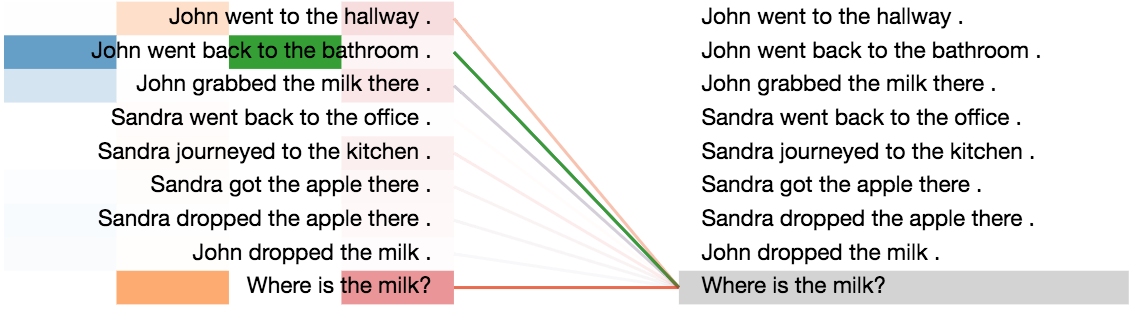
\includegraphics[height=1.3in]{04-part-03/chapter-06/figs_and_tables/figs_attention_babi/e3-step4}
        \caption{Step 4}
    \end{subfigure}
    \end{minipage}
    \caption{\label{fig:ex3}Visualization of the attention distributions, when encoding the question: \emph{``Where is the milk?''}.}
\end{figure}

\afterpage{\clearpage}

\begin{figure}[!h]
\begin{minipage}{\textwidth}
\fontsize{8}{8}\fontfamily{pcr}\selectfont
\begin{tabular}{l l}
\textbf{An example from tasks 3}: & \textbf{(requiring three supportive facts to solve)}\\
\\

\textbf{Story}: & \\
Mary got the milk. \\
& John moved to the bedroom. \\
& Daniel journeyed to the office. \\
& John grabbed the apple there. \\
& John got the football. \\
& John journeyed to the garden. \\
& Mary left the milk. \\
& John left the football. \\
& Daniel moved to the garden. \\
& Daniel grabbed the football. \\
& Mary moved to the hallway. \\
& Mary went to the kitchen. \\
& John put down the apple there. \\
& John picked up the apple. \\
& Sandra moved to the hallway. \\
& Daniel left the football there. \\
& Daniel took the football. \\
& John travelled to the kitchen. \\
& Daniel dropped the football. \\
& John dropped the apple. \\
& John grabbed the apple. \\
& John went to the office. \\
& Sandra went back to the bedroom. \\
& Sandra took the milk. \\
& John journeyed to the bathroom. \\
& John travelled to the office. \\
& Sandra left the milk. \\
& Mary went to the bedroom. \\
& Mary moved to the office. \\
& John travelled to the hallway. \\
& Sandra moved to the garden. \\
& Mary moved to the kitchen. \\
& Daniel took the football. \\
& Mary journeyed to the bedroom. \\
& Mary grabbed the milk there. \\
& Mary discarded the milk. \\
& John went to the garden. \\
& John discarded the apple there. \\
\\
\textbf{Question}: & \\
& Where was the apple before the bathroom? \\
\textbf{Model's output}: & \\
& office
\end{tabular}
\end{minipage}
\end{figure}
\begin{figure}[h!]\ContinuedFloat
\begin{minipage}{\textwidth}
    \centering
    \begin{subfigure}[t]{\textwidth}
        \centering
        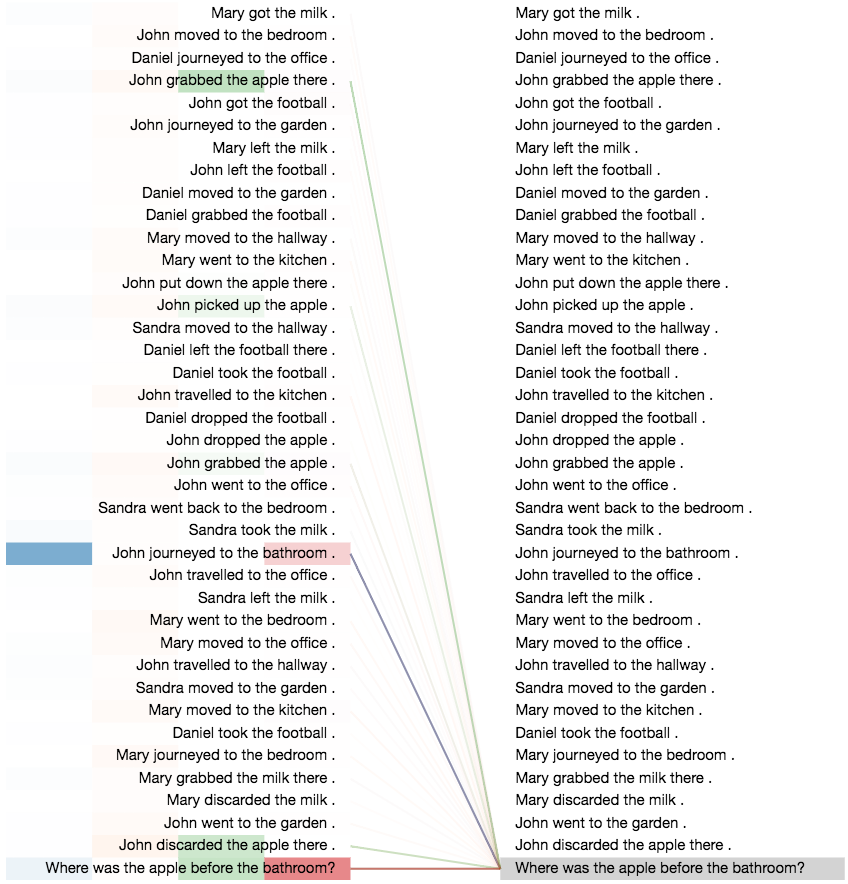
\includegraphics[height=4.2in]{04-part-03/chapter-06/figs_and_tables/figs_attention_babi/e4-step1}
        \caption{Step 1}
    \end{subfigure}%
    \hfill \hfill
    \begin{subfigure}[t]{\textwidth}
        \centering
        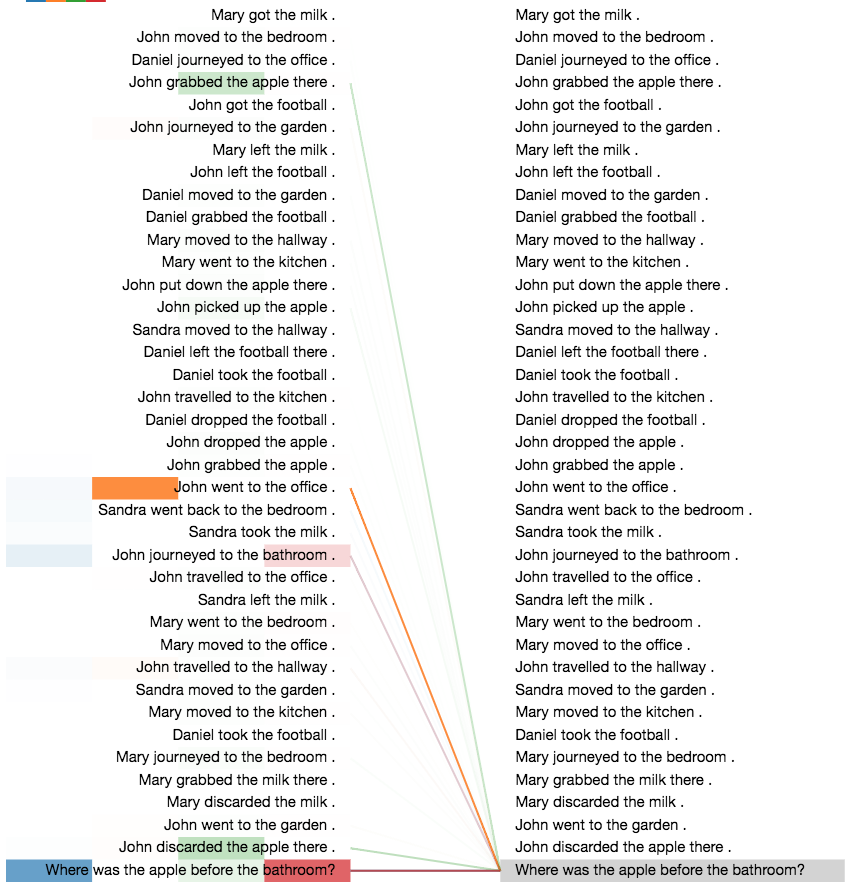
\includegraphics[height=4.2in, trim={0 0 0 0.1cm},clip]{04-part-03/chapter-06/figs_and_tables/figs_attention_babi/e4-step2}
        \caption{Step 2}
    \end{subfigure}
\end{minipage}
\end{figure}
\begin{figure}[h!]\ContinuedFloat
\begin{minipage}{\textwidth}\ContinuedFloat
    \begin{subfigure}[t]{\textwidth}
        \centering
        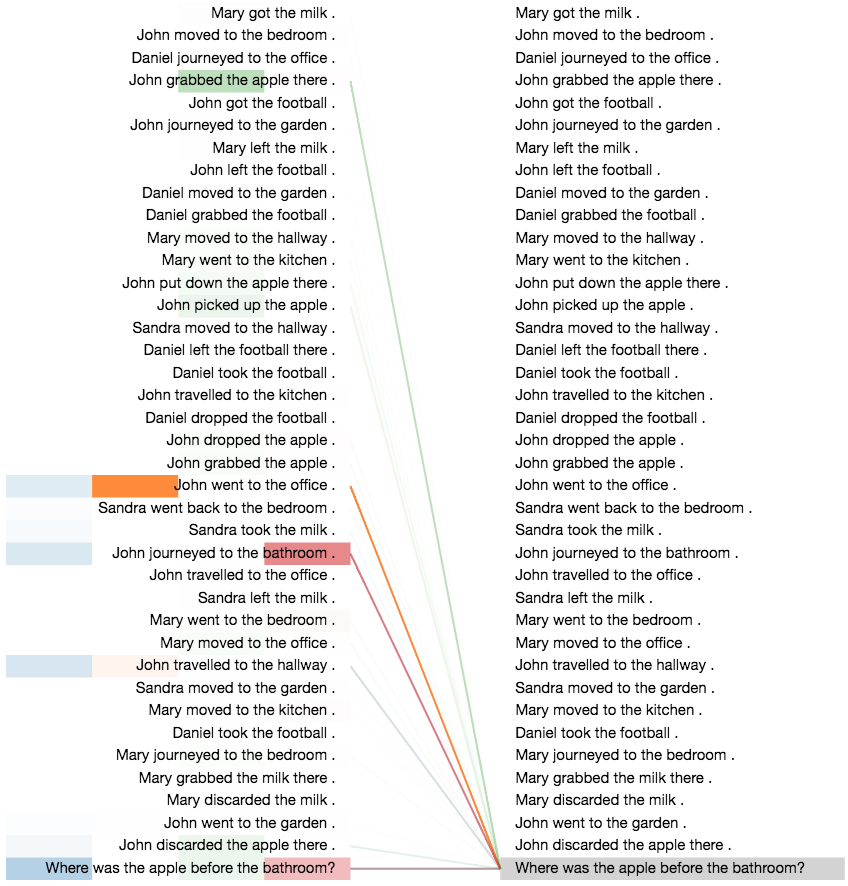
\includegraphics[height=4.2in]{04-part-03/chapter-06/figs_and_tables/figs_attention_babi/e4-step3}
        \caption{Step 3}
    \end{subfigure}
    \hfill \hfill 
    \begin{subfigure}[t]{\textwidth}
        \centering
        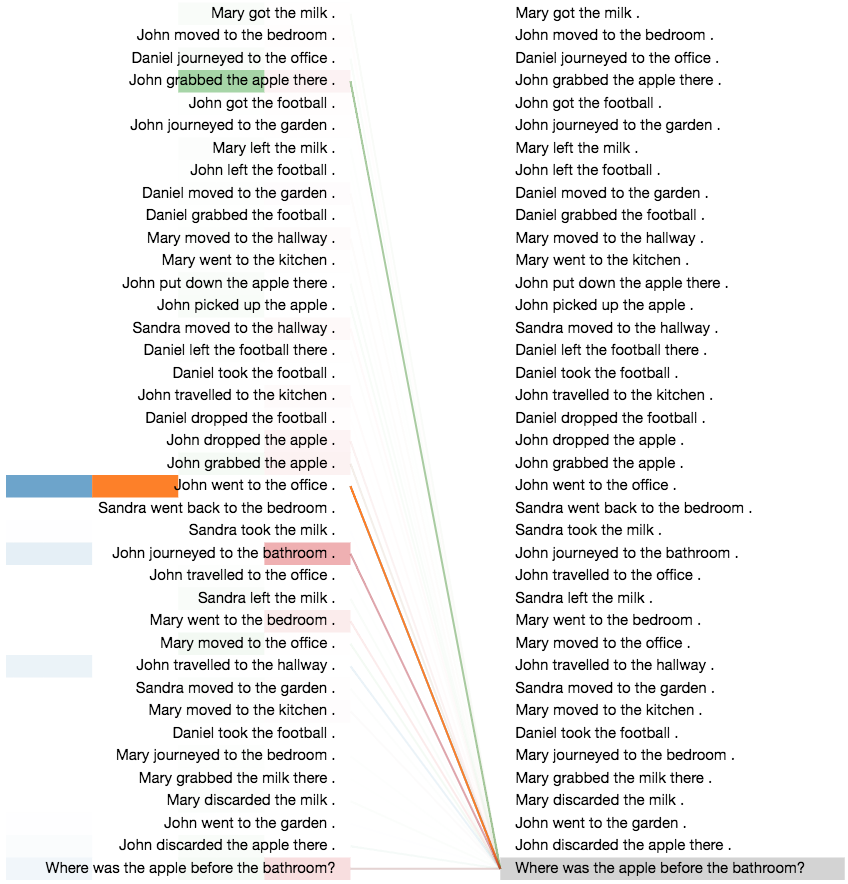
\includegraphics[height=4.2in]{04-part-03/chapter-06/figs_and_tables/figs_attention_babi/e4-step4}
        \caption{Step 4}
    \end{subfigure}
    \caption{\label{fig:ex4}Visualization of the attention distributions, when encoding the question: \emph{``Where was the apple before the bathroom?''}.}
\end{minipage}
\end{figure}